% ======= CLaNN: FE stretch -> dataset -> CLaNN arch (vertical) -> S -> Train -> (g,H) -> FE inflation =======
% Требует: \usepackage{tikz} \usetikzlibrary{arrows.meta,positioning,fit}
\begin{tikzpicture}[
  font=\small, node distance=8mm and 14mm, >={Latex},
  box/.style={draw, rounded corners, align=center, minimum height=8mm, inner sep=2mm},
  thinbox/.style={draw, rounded corners, align=center, minimum height=6mm, inner sep=1.2mm, text width=52mm},
  inpin/.style={circle, draw, minimum size=5.2mm},
  hid/.style={circle, draw, minimum size=6mm},
  title/.style={font=\bfseries},
  dashedarrow/.style={->, dashed},
  boxL/.style={box, fill=blue!6},
  boxM/.style={box, fill=green!6},
  boxR/.style={box, fill=orange!10},
  trainbox/.style={box, fill=purple!8}
]

% ---------------- Simplified pipeline (3 columns, orthogonal arrows) ----------------
% LEFT COLUMN
\node[boxL, minimum width=46mm, minimum height=32mm] (fe) {FE-растяжение\\ \scriptsize протоколы $p$\\[2pt]
  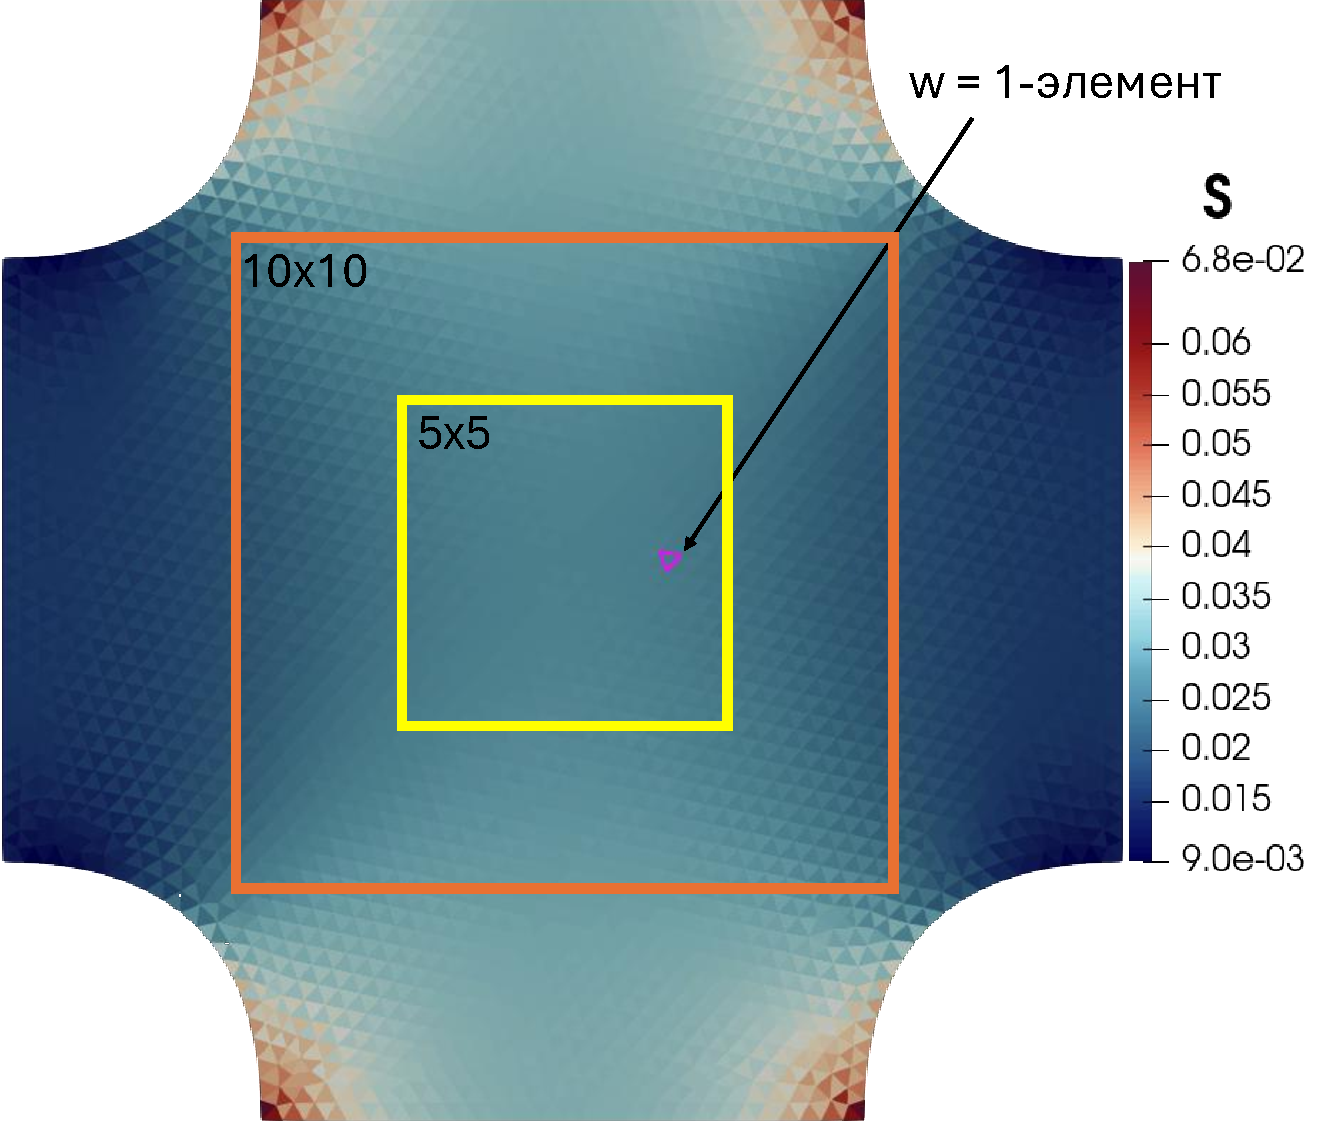
\includegraphics[width=0.3\linewidth]{img/Numerical/malt_window.pdf}};
\node[boxL, below=8mm of fe, minimum width=46mm] (data) {Сбор данных\\ $D(p,w)=\{(C,S)\}$};

% MIDDLE COLUMN
\node[boxM, right=28mm of fe, minimum width=54mm] (xi) {деформация Лапласа\\ $\boldsymbol{\xi}=\boldsymbol{\xi}(C)$};
\node[boxM, below=8mm of xi, minimum width=54mm] (arch) {Архитектура CLaNN\\ $\psi_{\rm phys}(\boldsymbol{\xi})$};
\node[boxM, below=8mm of arch, minimum width=54mm] (smap) {Автодифференцирование \\ $S=\partial\psi/\partial C$};
\node[trainbox, below=8mm of smap, minimum width=54mm] (train) {Обучение\\ $L=\|\vect S_{pred}-\vect S\|_{L2}$ (Adam)};

% RIGHT COLUMN
\node[boxR, right=28mm of arch, minimum width=50mm] (gh) {Производные\\ $g(\xi),\ H(\xi)$};
\node[boxR, below=8mm of gh, minimum width=50mm, minimum height=36mm] (infl) {FE-раздутие\\ рексация + Ньютон\\[2pt]
  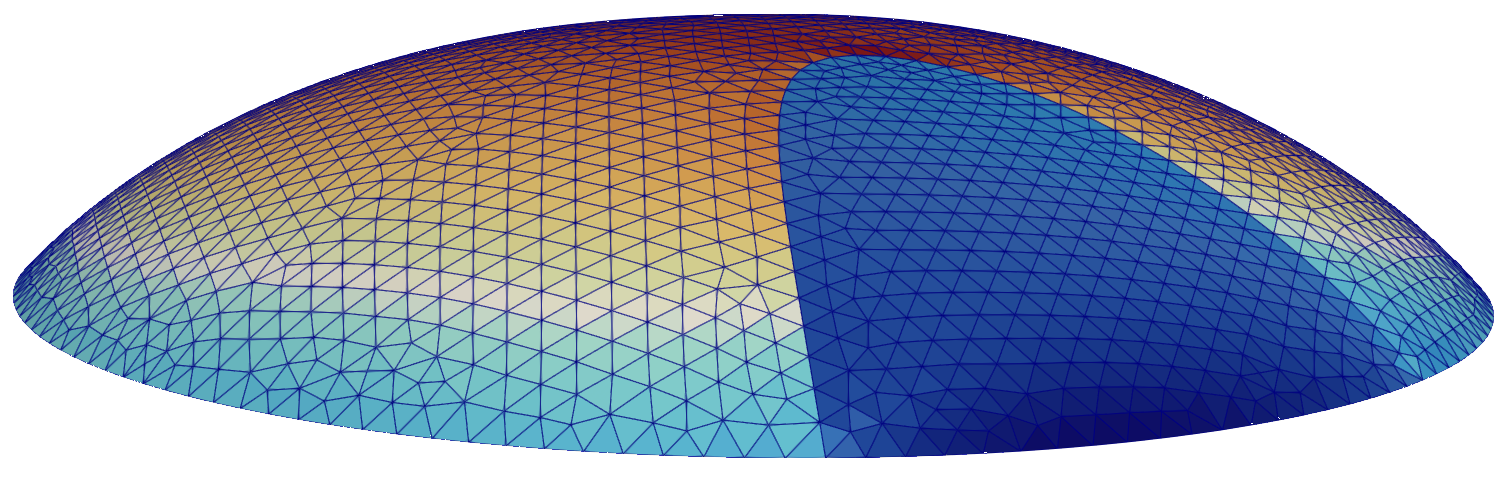
\includegraphics[width=0.3\linewidth]{img/Numerical/het/plane.png}};

% ORTHOGONAL ARROWS
\draw[->] (fe) -- (data);
% вилка от датасета: одна ветвь к деформации, другая — к обучению
\path (data.east) -- ++(10mm,0) coordinate (datasplit);
\draw[->] (data.east) -- (datasplit) |- (xi.west);
\draw[->] (datasplit) |- (train.west);
\draw[->] (xi) -- (arch);
\draw[->] (arch) -- (smap);
\draw[->] (smap) -- (train);
\draw[->] (arch.east) -- (gh.west);
\draw[->] (gh.south) -- (infl.north);
% пунктир: обновление параметров из обучения обратно в архитектуру (слева)
\draw[dashedarrow] (train.west) -- ++(-8mm,0) |- (arch.west);

\end{tikzpicture}
